% \section{Introduction to the Appendices}

% The Appendices is where you are enabled to present any additional or supplementary information relevant to your study, yet do not require highlighting within the actual paper, either because of its trivial nature or volume. These may in the form of figures, tables, or additional text detailing specific aspects about or related to the study.

% \section{Sample Questions for Different Studies}
% The following table presents three sample studies, as well as the guide questions that may help direct the discussion in each section of the paper. You may use this as another reference in writing your paper.

%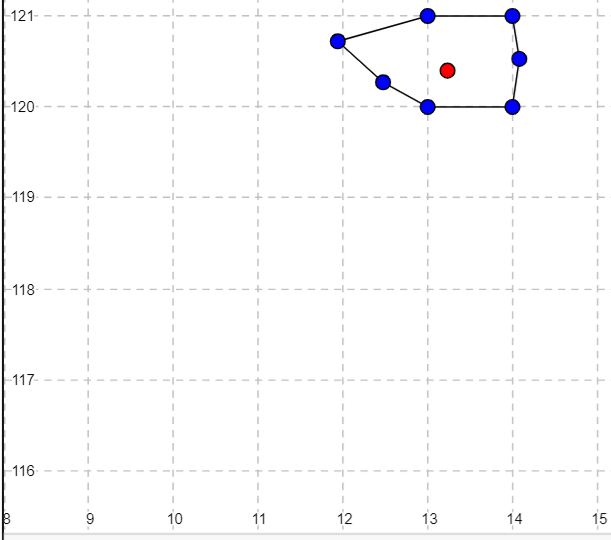
\includegraphics[width=\textwidth]{SampleThesisQuery.PNG}

\chapter{Geolocation Query Visualization}



\begin{figure}[hbt!]
    %\centering
    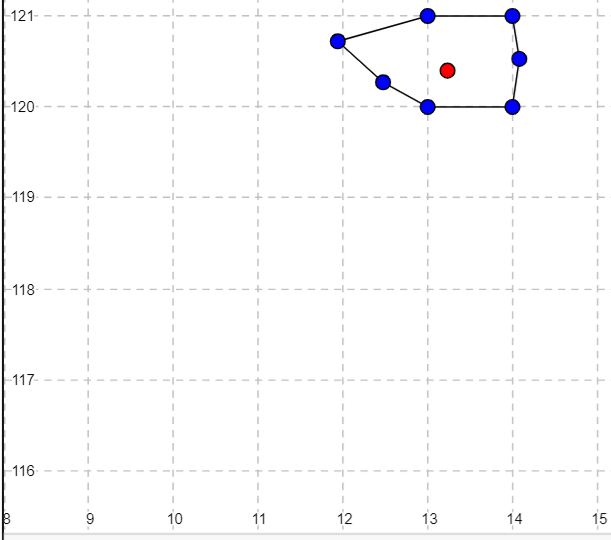
\includegraphics[width=\textwidth, height=\textheight,keepaspectratio]{SampleThesisQuery.PNG}
    \caption{Sample Query Visualization. Red point indicates approximated tweet. Blue points indicate already-geolocated tweets.}
    %\label{fig:my_label}
\end{figure}

